% !TeX root = ../../tfg.tex
% !TeX encoding = utf8
%
%*******************************************************
% Qué es el aprendizaje automático
%*******************************************************

\section{Concepto de aprendizaje}\label{ch:Aprendizaje}

Las redes neuronales son un tipo de algoritmos de Aprendizaje Automático. Por ello, no sería prudente exponer la historia de las redes neuronales sin dar en primer lugar una nociones básicas del área del saber a la que pertenecen.

El término de Aprendizaje Automático 
\cite{hisour} 
fue acuñado en 1959 por Arthur Samuel 
para hacer referencia a los sistemas informáticos que 
pueden \textit{aprender} por sí mismos, es decir, mejorar su 
eficacia y rendimiento de forma autónoma a partir de los datos, 
sin que en esas mejoras intervenga un programador.

\begin{marginfigure}
    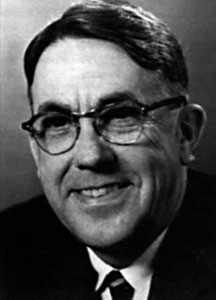
\includegraphics[width=\marginparwidth]{introduccion_redes_neuronales/aprendizaje_introduccion/arthur_samuel.jpg}
    \caption{Arthur L. Samuel (1901-1990) }
    \cite{samuel-wikipedia}
    \small
     se graduó en Ingeniería Electrónica en el MIT. 
     Trabajó en los laboratorios Bell, la Universidad de Illinois,
      en IBM y en la Universidad de Stanford (1966). 
      Fue un pionero de los videojuegos y la inteligencia artificial. 
      Popularizó el término \textit{Machine Learning} en 1959. 
      Implementó una IA para jugar a las damas, el primer caso  
      de éxito en aprendizaje automático. Contribuyó notablemente 
      en el desarrollo de TeX.
\end{marginfigure}

Fue en 1997 cuando Tom Mitchell propuso una definición 
más formal de aprendizaje 
\cite{tom-michell-machine-learning}, 
aproximada a la dada en el libro \textit{Learning from data}
\cite{learning-from-data-1-2}, que expondremos en seguida.

El aprendizaje es un proceso por el cual se estima una dependencia desconocida 
(input-output) o la estructura de un sistema a partir de un número finito de 
observaciones.  El aprendizaje se compone de tres elementos principales: 

\begin{itemize}
    \item Un generador o función de distribución de la cual se extraen 
    vectores aleatorios 
    $x \in \mathbb R^ n$ 
    que dependen de una función de densidad desconocida \footnote{De hecho, encontrar esta función resolvería el problema de aprendizaje}.
    
    \item Un sistema que produce un vector de salida $y$ por cada entrada del vector $x$ a partir del valor fijo $p(y|x)$, que es desconocido también. 
    
    \item Una \textit{learning machine}, que en el caso más general no es  más que un conjunto de funciones abstractas cuyos elementos son de la forma $f(x,w), w\in \omega$.
\end{itemize}

\begin{marginfigure}
    
\includegraphics[width=\marginparwidth]{introduccion_redes_neuronales/aprendizaje_introduccion/tom_mitchell.jpg}
   \caption{Tom M. Mitchell}
   \small
    Tom M. Mitchell
     \cite{mitchell-wikipedia} 
    (1951) estudió Ingeniería Electrónica en el MIT, 
    se doctoró en la Universidad de Stanford y ejerce en la Universidad de Carnegie Mellon. 
    Es conocido por su libro 
    de texto Machine Learning. Ha recibido numerosas condecoraciones y 
   participa en asociaciones que promueven la ciencia y la ingeniería.
\end{marginfigure}



Así pues, el objetivo del aprendizaje automático es encontrar una función que se aproxime a la función de densidad desconocida.

Por lo general la teoría se fundamenta en minimizar el error de estimadores, como el error cuadrático medio, ya que este se trata de un UMVUE  (estimador insesgado de mínima varianza). 

$$ECM = \frac{1}{n} \sum_{i=0} ^n (f(x_i) - y_i)^2,$$

donde $f(x_i)$ representa la predicción y $y_i$ la etiqueta de entrenamiento de $x_i$, es decir, su valor real. 

% Componentes del aprendizaje   
\subsection{Componentes del aprendizaje}  

(Información proveniente del capítulo 1 \cite{MostafaLearningFromData})
Los principales componentes del aprendizaje son: 

\begin{itemize}
    \item Una entrada $x$. 
    \item Una función objetivo ideal y desconocida
     $f: \mathcal X \longrightarrow \mathcal{Y}$. 
     Donde  $\mathcal X$ es el espacio de entrada al que pertenecen las entradas $x$ y $\mathcal{Y}$ el espacio de salida. 
    \item Un conjunto de datos de entrenamiento $\mathcal D.$
    \item Un algoritmo de aprendizaje que consiste en seleccionar una fórmula $g: \mathcal X \longrightarrow \mathcal{Y}$ que aproxime $f$. La fórmula $g$ pertenece 
    a un conjunto $\mathcal H$ de hipótesis. 
\end{itemize}

En nuestro caso $\mathcal{H}$ será el conjunto de todas las posibles redes neuronales y $g$ la red neuronal seleccionada. 


% Tipos de aprendizaje 
\subsection{Tipos de aprendizaje}  

(Información proveniente del capítulo 1 \cite{MostafaLearningFromData})

El aprendizaje a partir de los datos consiste en el uso de un 
un conjunto de observaciones con el fin de descubrir un patrón, modelo o ley del proceso subyacente. 

En función de ciertas características del conjunto de datos se 
tienen distintos tipos de aprendizaje.  

\subsubsection{Aprendizaje supervisado}
Cuando el conjunto de datos de entrenamiento contiene de manera explícita lo que es una salida correcta respecto a una entrada estamos frente a un caso de \textbf{aprendizaje no supervisado}.   

Un ejemplo sería el reconocimiento de dígitos  manuscritos donde cada imagen de un dígito tiene asociado cuál es. 


\subsubsection{Aprendizaje por refuerzo}  
Se trata de un problema de aprendizaje por refuerzo 
cuando conjunto de datos de entrenamiento no explicita la salida, en su lugar contiene posibles salidas junto a la bondad de éstas. 

Pongamos por ejemplo que se quiere enseñar a un sistema a jugar
a las damas; de todo el espacio de jugadas posibles, se conocerían tan solo el resultado de algunas situaciones, por ejemplo en la que uno de los jugadores ha ganado.  

\subsubsection{Aprendizaje no supervisado}  

En este tipo de aprendizaje, los datos de entrenamiento tampoco contienen ninguna información de la salida.
 Tan solo se tienen los datos de entrada. El \textbf{aprendizaje no supervisado} 
 consiste en la tarea de encontrar patrones y estructuras en los datos de entrada, 
 así como de crear una una abstracción de los datos.  


Las redes neuronales son partícipes en los tres tipos de aprendizaje 
recién mencionados
\cite{8612259}, \cite{DBLP:journals/corr/BakerGNR16}, \cite{10.5555/2955491.2955578}. Sin embargo centraremos nuestro estudio en el caso 
de aprendizaje supervisado. 

Además, podríamos clasificar también el tipo de problemas en función del tipo de salida requerida (capítulo 4 pag 179
\cite{BishopPaterRecognition}), en regresión, clasificación o probabilistas. 
Dada una salida cualquiera, la adaptación de esta a un dominio concreto se consigue por medio de funciones 
no lineales, las cuales denotamos como \textbf{funciones de activación}. 